% Options for packages loaded elsewhere
\PassOptionsToPackage{unicode}{hyperref}
\PassOptionsToPackage{hyphens}{url}
%
\documentclass[
]{article}
\usepackage{amsmath,amssymb}
\usepackage{lmodern}
\usepackage{ifxetex,ifluatex}
\ifnum 0\ifxetex 1\fi\ifluatex 1\fi=0 % if pdftex
  \usepackage[T1]{fontenc}
  \usepackage[utf8]{inputenc}
  \usepackage{textcomp} % provide euro and other symbols
\else % if luatex or xetex
  \usepackage{unicode-math}
  \defaultfontfeatures{Scale=MatchLowercase}
  \defaultfontfeatures[\rmfamily]{Ligatures=TeX,Scale=1}
\fi
% Use upquote if available, for straight quotes in verbatim environments
\IfFileExists{upquote.sty}{\usepackage{upquote}}{}
\IfFileExists{microtype.sty}{% use microtype if available
  \usepackage[]{microtype}
  \UseMicrotypeSet[protrusion]{basicmath} % disable protrusion for tt fonts
}{}
\makeatletter
\@ifundefined{KOMAClassName}{% if non-KOMA class
  \IfFileExists{parskip.sty}{%
    \usepackage{parskip}
  }{% else
    \setlength{\parindent}{0pt}
    \setlength{\parskip}{6pt plus 2pt minus 1pt}}
}{% if KOMA class
  \KOMAoptions{parskip=half}}
\makeatother
\usepackage{xcolor}
\IfFileExists{xurl.sty}{\usepackage{xurl}}{} % add URL line breaks if available
\IfFileExists{bookmark.sty}{\usepackage{bookmark}}{\usepackage{hyperref}}
\hypersetup{
  pdftitle={WKCLIMAD},
  hidelinks,
  pdfcreator={LaTeX via pandoc}}
\urlstyle{same} % disable monospaced font for URLs
\usepackage[margin=1in]{geometry}
\usepackage{color}
\usepackage{fancyvrb}
\newcommand{\VerbBar}{|}
\newcommand{\VERB}{\Verb[commandchars=\\\{\}]}
\DefineVerbatimEnvironment{Highlighting}{Verbatim}{commandchars=\\\{\}}
% Add ',fontsize=\small' for more characters per line
\usepackage{framed}
\definecolor{shadecolor}{RGB}{248,248,248}
\newenvironment{Shaded}{\begin{snugshade}}{\end{snugshade}}
\newcommand{\AlertTok}[1]{\textcolor[rgb]{0.94,0.16,0.16}{#1}}
\newcommand{\AnnotationTok}[1]{\textcolor[rgb]{0.56,0.35,0.01}{\textbf{\textit{#1}}}}
\newcommand{\AttributeTok}[1]{\textcolor[rgb]{0.77,0.63,0.00}{#1}}
\newcommand{\BaseNTok}[1]{\textcolor[rgb]{0.00,0.00,0.81}{#1}}
\newcommand{\BuiltInTok}[1]{#1}
\newcommand{\CharTok}[1]{\textcolor[rgb]{0.31,0.60,0.02}{#1}}
\newcommand{\CommentTok}[1]{\textcolor[rgb]{0.56,0.35,0.01}{\textit{#1}}}
\newcommand{\CommentVarTok}[1]{\textcolor[rgb]{0.56,0.35,0.01}{\textbf{\textit{#1}}}}
\newcommand{\ConstantTok}[1]{\textcolor[rgb]{0.00,0.00,0.00}{#1}}
\newcommand{\ControlFlowTok}[1]{\textcolor[rgb]{0.13,0.29,0.53}{\textbf{#1}}}
\newcommand{\DataTypeTok}[1]{\textcolor[rgb]{0.13,0.29,0.53}{#1}}
\newcommand{\DecValTok}[1]{\textcolor[rgb]{0.00,0.00,0.81}{#1}}
\newcommand{\DocumentationTok}[1]{\textcolor[rgb]{0.56,0.35,0.01}{\textbf{\textit{#1}}}}
\newcommand{\ErrorTok}[1]{\textcolor[rgb]{0.64,0.00,0.00}{\textbf{#1}}}
\newcommand{\ExtensionTok}[1]{#1}
\newcommand{\FloatTok}[1]{\textcolor[rgb]{0.00,0.00,0.81}{#1}}
\newcommand{\FunctionTok}[1]{\textcolor[rgb]{0.00,0.00,0.00}{#1}}
\newcommand{\ImportTok}[1]{#1}
\newcommand{\InformationTok}[1]{\textcolor[rgb]{0.56,0.35,0.01}{\textbf{\textit{#1}}}}
\newcommand{\KeywordTok}[1]{\textcolor[rgb]{0.13,0.29,0.53}{\textbf{#1}}}
\newcommand{\NormalTok}[1]{#1}
\newcommand{\OperatorTok}[1]{\textcolor[rgb]{0.81,0.36,0.00}{\textbf{#1}}}
\newcommand{\OtherTok}[1]{\textcolor[rgb]{0.56,0.35,0.01}{#1}}
\newcommand{\PreprocessorTok}[1]{\textcolor[rgb]{0.56,0.35,0.01}{\textit{#1}}}
\newcommand{\RegionMarkerTok}[1]{#1}
\newcommand{\SpecialCharTok}[1]{\textcolor[rgb]{0.00,0.00,0.00}{#1}}
\newcommand{\SpecialStringTok}[1]{\textcolor[rgb]{0.31,0.60,0.02}{#1}}
\newcommand{\StringTok}[1]{\textcolor[rgb]{0.31,0.60,0.02}{#1}}
\newcommand{\VariableTok}[1]{\textcolor[rgb]{0.00,0.00,0.00}{#1}}
\newcommand{\VerbatimStringTok}[1]{\textcolor[rgb]{0.31,0.60,0.02}{#1}}
\newcommand{\WarningTok}[1]{\textcolor[rgb]{0.56,0.35,0.01}{\textbf{\textit{#1}}}}
\usepackage{graphicx}
\makeatletter
\def\maxwidth{\ifdim\Gin@nat@width>\linewidth\linewidth\else\Gin@nat@width\fi}
\def\maxheight{\ifdim\Gin@nat@height>\textheight\textheight\else\Gin@nat@height\fi}
\makeatother
% Scale images if necessary, so that they will not overflow the page
% margins by default, and it is still possible to overwrite the defaults
% using explicit options in \includegraphics[width, height, ...]{}
\setkeys{Gin}{width=\maxwidth,height=\maxheight,keepaspectratio}
% Set default figure placement to htbp
\makeatletter
\def\fps@figure{htbp}
\makeatother
\setlength{\emergencystretch}{3em} % prevent overfull lines
\providecommand{\tightlist}{%
  \setlength{\itemsep}{0pt}\setlength{\parskip}{0pt}}
\setcounter{secnumdepth}{-\maxdimen} % remove section numbering
\ifluatex
  \usepackage{selnolig}  % disable illegal ligatures
\fi

\title{WKCLIMAD}
\author{}
\date{\vspace{-2.5em}}

\begin{document}
\maketitle

{
\setcounter{tocdepth}{2}
\tableofcontents
}
\hypertarget{wkclimad-overview}{%
\section{1. WKCLIMAD Overview}\label{wkclimad-overview}}

This repository contains R code and Rdata files for working with
WKCLIMAD data and responses. WKCLIMAD is an ICES workshop aimed at
exploring how can the short-, medium-, and long-term influences of
climate change on aquaculture, fisheries, and ecosystems be accounted
for in ICES Advice.

The workshop is chaired by: Mark Dickey-Collas, Kirstin Kari Holsman,
and Michael Rust. More information can be found
here:\url{https://www.ices.dk/community/groups/Pages/WKCLIMAD.aspx}

\hypertarget{summary}{%
\subsection{Summary:}\label{summary}}

As managers, policy-makers, and other stakeholders become increasingly
aware of the need to consider climate impacts, this workshop will
develop a proposal for an operational climate-aware advisory framework.
Experts are invited to join WKCLIMAD to review the recent and emergent
analyses of key climate hazards to aquaculture, fisheries, and
ecosystems.

The workshop will outline actionable strategies and approaches that can
be taken to promote resiliency in fisheries, aquaculture, and
ecosystems. It will scope the next steps for an operational approach,
expanding the relevant aspects of climate change that impact management
decisions in fisheries, aquaculture and ecosystems.

The kick off meeting will take place on the 21 June 2021, and
participants will work via correspondence prior to the online meetings
taking place 29--30 September and 18--20 October 2021.

Registration is now closed. Selected participants will be announced by
15 June 2021.

We expect this to be a popular workshop and therefore may have to limit
the number of participants. If the workshop is oversubscribed, ICES
reserves the right, in consultation with the workshop chairs, to select
the final workshop participants based on their expertise, and equitable
makeup of the workshop.

\hypertarget{code-overview}{%
\section{2. Code overview}\label{code-overview}}

In August 2021 multiple experts provided a rapid assessment of climate
impacts via a Delphi approach. The code below analyses the output from
that activity and produces the plots and results summarized in the
WKCLIMAD report. The code below will generate the following plot:

\begin{figure}
\centering
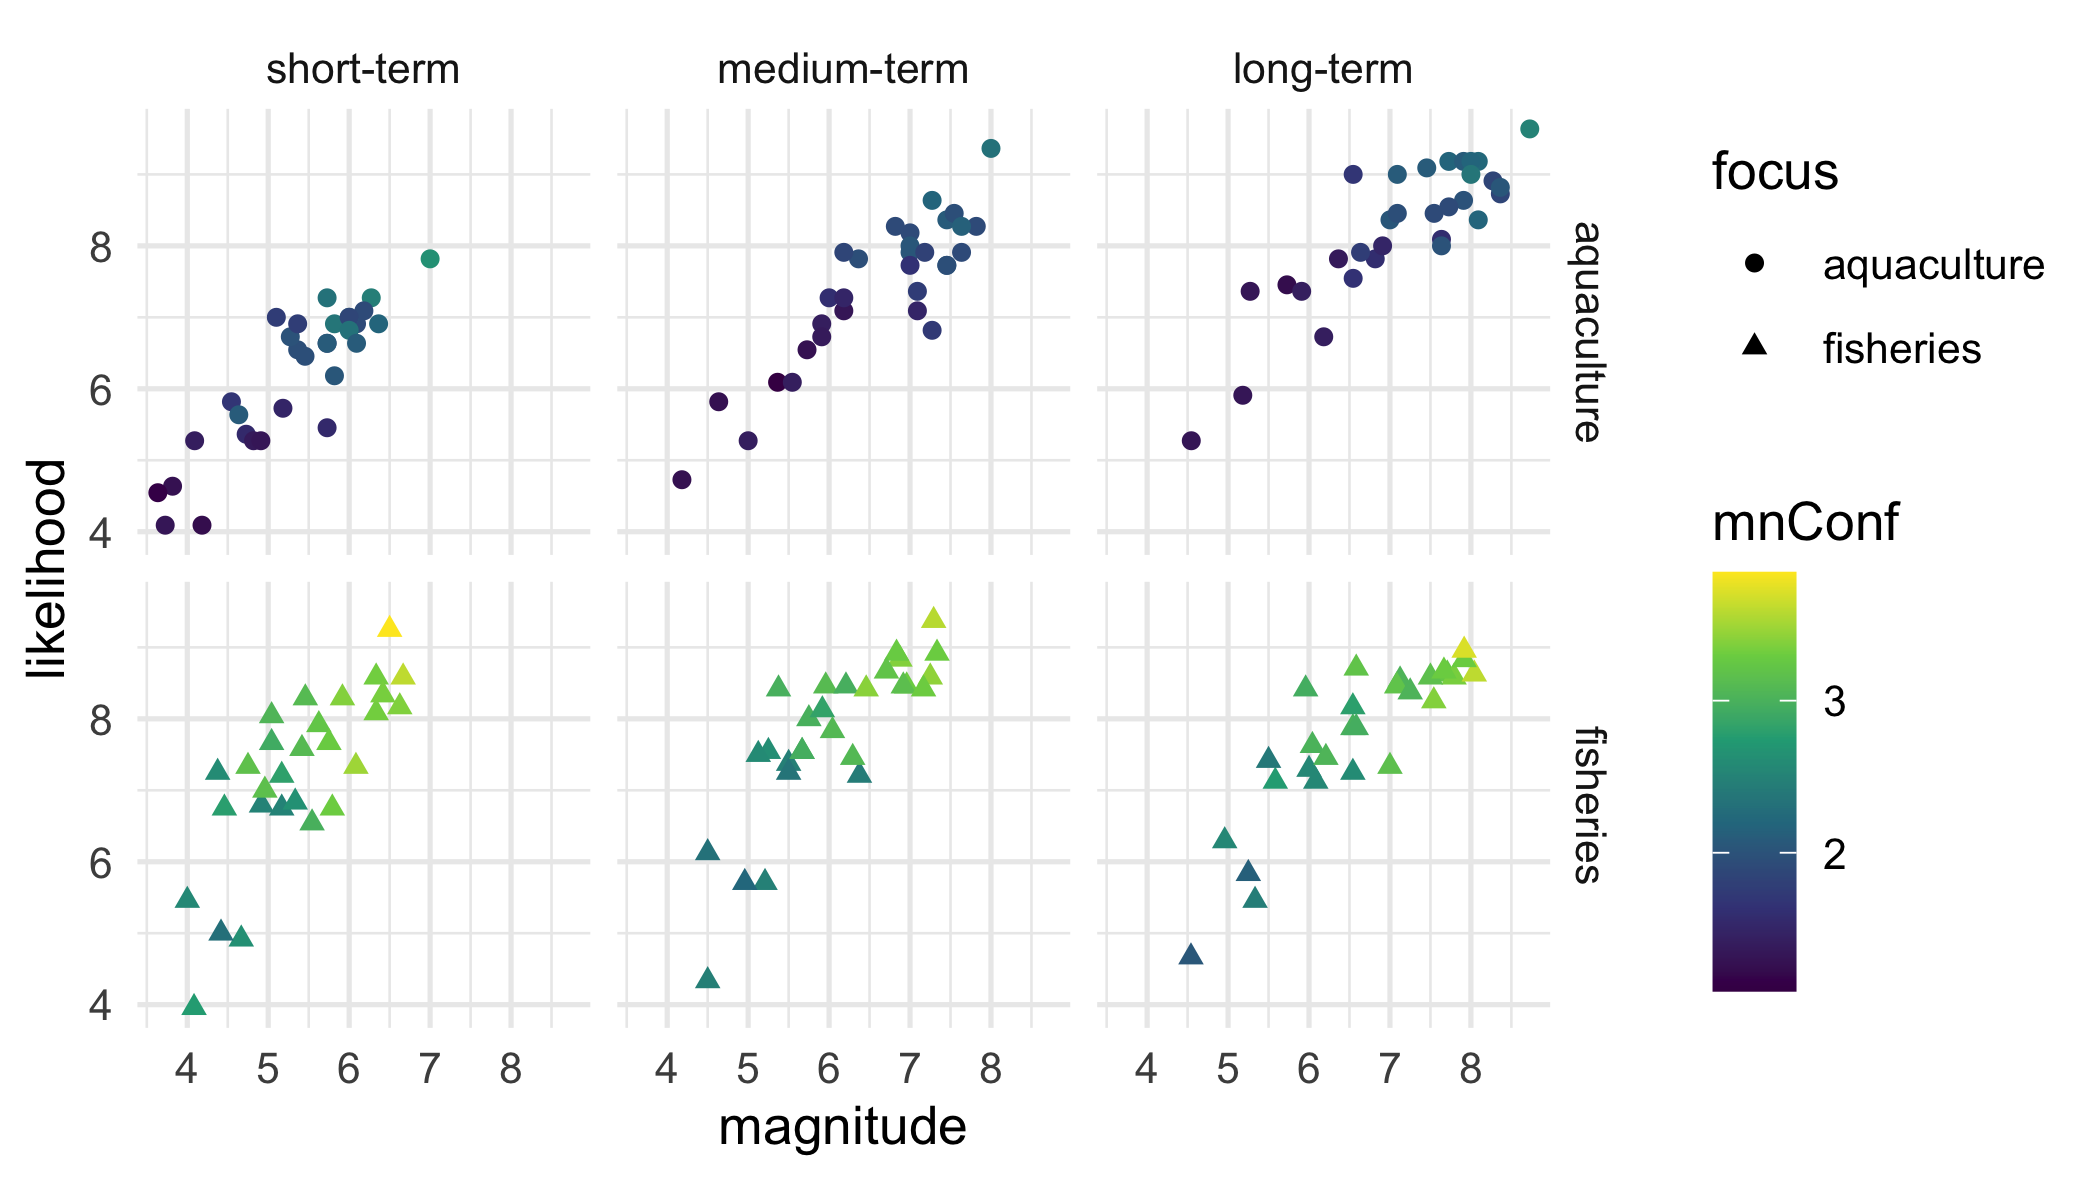
\includegraphics[width=0.65\textwidth,height=\textheight]{Figs/Fig1.png}
\caption{Results of the first round of Delphi surveys.}
\end{figure}

\begin{Shaded}
\begin{Highlighting}[]
   \CommentTok{\# loads packages, data, setup, etc.}
    \FunctionTok{suppressWarnings}\NormalTok{(}\FunctionTok{source}\NormalTok{(}\StringTok{"R/make.R"}\NormalTok{))}
    
    \CommentTok{\# reshape the data into long{-}format:}
    \CommentTok{\# {-}{-}{-}{-}{-}{-}{-}{-}{-}{-}{-}{-}{-}{-}{-}{-}{-}{-}{-}{-}{-}{-}{-}{-}{-}{-}{-}{-}{-}{-}{-}{-}{-}{-}{-}{-}{-}{-}}
\NormalTok{    long\_a }\OtherTok{\textless{}{-}} \FunctionTok{getData}\NormalTok{(aqua\_dat)}
\NormalTok{    long\_f }\OtherTok{\textless{}{-}} \FunctionTok{getData}\NormalTok{(fish\_dat)}
\NormalTok{    long\_a}\SpecialCharTok{$}\NormalTok{focus }\OtherTok{\textless{}{-}} \StringTok{"aquaculture"}
\NormalTok{    long\_f}\SpecialCharTok{$}\NormalTok{focus }\OtherTok{\textless{}{-}} \StringTok{"fisheries"}
    
    \CommentTok{\# combine into single long format:}
\NormalTok{    long }\OtherTok{\textless{}{-}} \FunctionTok{rbind}\NormalTok{(long\_a,long\_f)}
    
    \CommentTok{\# summarize across participants:}
\NormalTok{    smry }\OtherTok{\textless{}{-}}\NormalTok{ long}\SpecialCharTok{\%\textgreater{}\%}\FunctionTok{group\_by}\NormalTok{(focus,category,time\_period,type)}\SpecialCharTok{\%\textgreater{}\%}\FunctionTok{summarise}\NormalTok{(}
      \AttributeTok{mn =} \FunctionTok{mean}\NormalTok{(value.x,}\AttributeTok{na.rm=}\NormalTok{T),}
      \AttributeTok{sd =} \FunctionTok{sd}\NormalTok{ (value.x,}\AttributeTok{na.rm=}\NormalTok{T),}
      \AttributeTok{n  =} \FunctionTok{length}\NormalTok{(value.x),}
      \AttributeTok{median =} \FunctionTok{median}\NormalTok{(value.x,}\AttributeTok{na.rm=}\NormalTok{T),}
      \AttributeTok{mn\_conf =} \FunctionTok{mean}\NormalTok{(conf\_n,}\AttributeTok{na.rm=}\NormalTok{T),}
      \AttributeTok{sd\_conf =} \FunctionTok{sd}\NormalTok{(conf\_n,}\AttributeTok{na.rm=}\NormalTok{T),}
      \AttributeTok{median\_conf =} \FunctionTok{median}\NormalTok{(conf\_n,}\AttributeTok{na.rm=}\NormalTok{T))}
\NormalTok{    smry}\SpecialCharTok{$}\NormalTok{type }\OtherTok{\textless{}{-}} \FunctionTok{factor}\NormalTok{(smry}\SpecialCharTok{$}\NormalTok{type)}
    
    \CommentTok{\# split mag and likelihood into columns:}
\NormalTok{    smry\_w    }\OtherTok{\textless{}{-}}\NormalTok{ tidyr}\SpecialCharTok{::}\FunctionTok{spread}\NormalTok{(smry}\SpecialCharTok{\%\textgreater{}\%}
                                 \FunctionTok{select}\NormalTok{(focus,time\_period,category,type, mn), }
                               \AttributeTok{key =}\NormalTok{ type, }\AttributeTok{value =}\NormalTok{ mn)}
\NormalTok{    smry\_conf }\OtherTok{\textless{}{-}}\NormalTok{ tidyr}\SpecialCharTok{::}\FunctionTok{spread}\NormalTok{(smry}\SpecialCharTok{\%\textgreater{}\%}
                                 \FunctionTok{select}\NormalTok{(focus,time\_period,category,type, mn\_conf), }
                               \AttributeTok{key =}\NormalTok{ type, }\AttributeTok{value =}\NormalTok{ mn\_conf)}
\NormalTok{    smry\_conf}\SpecialCharTok{$}\NormalTok{mnConf }\OtherTok{\textless{}{-}} \FunctionTok{apply}\NormalTok{(smry\_conf[,}\FunctionTok{c}\NormalTok{(}\StringTok{"likelihood"}\NormalTok{,}\StringTok{"magnitude"}\NormalTok{)],}\DecValTok{1}\NormalTok{,mean)}
    
\NormalTok{    smry\_w }\OtherTok{\textless{}{-}} \FunctionTok{merge}\NormalTok{(smry\_w, smry\_conf}\SpecialCharTok{\%\textgreater{}\%}
                      \FunctionTok{select}\NormalTok{(focus,time\_period,category, mnConf),}
                    \AttributeTok{by=}\FunctionTok{c}\NormalTok{(}\StringTok{"focus"}\NormalTok{,}\StringTok{"time\_period"}\NormalTok{,}\StringTok{"category"}\NormalTok{))}

\NormalTok{   p }\OtherTok{\textless{}{-}}  \FunctionTok{ggplot}\NormalTok{()}\SpecialCharTok{+}\FunctionTok{geom\_point}\NormalTok{(}\AttributeTok{data=}\NormalTok{smry\_w,}\FunctionTok{aes}\NormalTok{(}\AttributeTok{x     =}\NormalTok{ magnitude,}
                                             \AttributeTok{y     =}\NormalTok{ likelihood,}
                                             \AttributeTok{color =}\NormalTok{ mnConf,}
                                             \AttributeTok{shape =}\NormalTok{ focus))}\SpecialCharTok{+}
      \FunctionTok{scale\_color\_viridis\_c}\NormalTok{()}\SpecialCharTok{+}
      \FunctionTok{facet\_grid}\NormalTok{(focus}\SpecialCharTok{\textasciitilde{}}\NormalTok{time\_period)}\SpecialCharTok{+}\FunctionTok{theme\_minimal}\NormalTok{()}
     
    \CommentTok{\# geom\_text(data=smry\_w,aes(x=magnitude,y=likelihood,color=mnConf,shape=focus)}
\NormalTok{    sclr }\OtherTok{\textless{}{-}}\NormalTok{.}\DecValTok{75}
    \FunctionTok{png}\NormalTok{(}\StringTok{"Figs/Fig1.png"}\NormalTok{, }\AttributeTok{width =} \DecValTok{8}\SpecialCharTok{*}\NormalTok{sclr, }\AttributeTok{height =} \FloatTok{4.5}\SpecialCharTok{*}\NormalTok{sclr, }\AttributeTok{units =} \StringTok{"in"}\NormalTok{,}\AttributeTok{res =} \DecValTok{350}\NormalTok{)}
    \FunctionTok{print}\NormalTok{(p)}
    \FunctionTok{dev.off}\NormalTok{()}
    
\NormalTok{  p2 }\OtherTok{\textless{}{-}} \FunctionTok{ggplot}\NormalTok{()}\SpecialCharTok{+}\FunctionTok{geom\_point}\NormalTok{(}\AttributeTok{data=}\NormalTok{smry\_w,}
                            \FunctionTok{aes}\NormalTok{(}\AttributeTok{x=}\NormalTok{magnitude,}\AttributeTok{y=}\NormalTok{likelihood,}\AttributeTok{color=}\NormalTok{mnConf,}\AttributeTok{shape=}\NormalTok{focus))}\SpecialCharTok{+}
      \FunctionTok{scale\_color\_viridis\_c}\NormalTok{()}\SpecialCharTok{+}
      \FunctionTok{facet\_wrap}\NormalTok{(focus}\SpecialCharTok{\textasciitilde{}}\NormalTok{category)}\SpecialCharTok{+}\FunctionTok{theme\_minimal}\NormalTok{()}
       
    \FunctionTok{png}\NormalTok{(}\StringTok{"Figs/Fig2.png"}\NormalTok{, }\AttributeTok{width =} \DecValTok{8}\NormalTok{, }\AttributeTok{height =}\DecValTok{8}\NormalTok{, }\AttributeTok{units =} \StringTok{"in"}\NormalTok{,}\AttributeTok{res =} \DecValTok{350}\NormalTok{)}
    \FunctionTok{print}\NormalTok{(p2)}
    \FunctionTok{dev.off}\NormalTok{()}
   
\NormalTok{    datIN      }\OtherTok{\textless{}{-}}\NormalTok{ aqua\_dat}
   \CommentTok{\# add type (and range)}
\end{Highlighting}
\end{Shaded}


\end{document}
